\documentclass[specialist,
substylefile = spbu.rtx,
               subf,href,colorlinks=true, 12pt]{disser}

% \documentclass[specialist, substylefile = spbureport.rtx,
            %    subf,href,colorlinks=true, 12pt]{disser}

\usepackage[a4paper,
            mag=1000, includefoot,
            left=3cm, right=1.5cm, top=2cm, bottom=2cm, headsep=1cm, footskip=1cm]{geometry}

\usepackage[T1,T2A]{fontenc}
\usepackage{graphicx}
\graphicspath{ {images/} }
\usepackage{amsmath}
\usepackage{amsfonts}
\usepackage{amsthm} %for \newtheorem*
\usepackage{bm}
\usepackage[english,russian]{babel}

% \usepackage{polyglossia}
% \usepackage{fontspec}
% \setmainfont{Times New Roman}
% \setsansfont{Arial}
% \setmonofont{Courier New}

% Использовать полужирное начертание для векторов
\let\vec=\mathbf
% Включать подсекции в оглавление
\setcounter{tocdepth}{2}

% c++ code
\usepackage{listings}
\usepackage{xcolor}
\lstset { %
    language=C++,
    backgroundcolor=\color{black!5}, % set backgroundcolor
    basicstyle=\footnotesize,% basic font setting
}


\usepackage{hyperref}
\usepackage{relsize}
\usepackage{xspace}
\newcommand{\Cpp}{\texorpdfstring{\mbox{C\raisebox{.35ex}{\textsmaller[2]{++}}}\xspace}{C++}}
% \newcommand\Cpp{C\nolinebreak[4]\hspace{-.05em}\raisebox{.4ex}{\relsize{-3}{\textbf{++}}}}

% \newtheorem*{definition}{Определение}
% \newtheorem*{example}{Пример}
% \newtheorem*{hypothesis}{Гипотеза}
% \newtheorem*{question}{Вопрос}
% \newtheorem*{algorithm}{Алгоритм}

% \newcommand{\rank}{\mathsf{rank}\ }










\begin{document}


% \institution{Санкт-Петербургский государственный университет\\
%     Математико-механический факультет\\
%     Кафедра Статистического Моделирования
% }
% \title{«Научно-исследовательская работа» (семестр 7)}
% \topic{Разработка программных средств и решение задач принятия решений с помощью методов тропической математики.}
% \author{Ткаченко Егор Андреевич}
% \group{группа 19.Б04-мм}
% \sa       {Кривулин Николай Кимович}
% \sastatus {д.\,ф.-м.\,н., профессор}
% \city{Санкт-Петербург}
% \date{2023}

% \institution{Санкт-Петербургский государственный университет\\
%     Математико-механический факультет\\
%     Кафедра Статистического Моделирования
% }
% \title{«Научно-исследовательская работа» (семестр 8)}
% \topic{Разработка программных средств и решение задач принятия решений с помощью методов тропической математики.}
% \author{Ткаченко Егор Андреевич}
% \group{группа 19.Б04-мм}
% \sa       {Кривулин Николай Кимович}
% \sastatus {д.\,ф.-м.\,н., профессор}
% \city{Санкт-Петербург}
% \date{2023}
%     \maketitle


    \institution{%
        Санкт-Петербургский государственный университет\\
        Математико-механический факультет\\
        Кафедра Статистического Моделирования
    }

    \title{Выпускная квалификационная работа}

    % Тема
    \topic{Разработка программных средств и решение задач принятия решений с помощью методов тропической математики}

    % Автор
    \author{\textsc{Ткаченко} Егор Андреевич}

    \group{%
        Уровень образования: бакалавриат\\
        Направление 01.03.02 <<Прикладная математика и информатика>>\\
        Основная образовательная программа СВ.5004.2019 <<Прикладная математика и информатика>>
    }

    % Научный руководитель
    \sa       {Н.\,К.~Кривулин}
    \sastatus {Профессор, кафедра статистического моделирования\,\\
            д.\,ф.-м.\,н., профессор}

    % Рецензент
    \rev      {В.\,А.~Пархоменко}
    \revstatus{Старший преподаватель, Высшая школа интеллектуальных систем и суперкомпьютерных технологий СПбПУ Петра Великого}


    % Город и год
    \city{Санкт-Петербург}
    \date{\number\year}

    \maketitle

    %%
    %% Titlepage in English
    %%
    %
    \institution{%
        Saint Petersburg State University \\
        Applied Mathematics and Computer Science
    }
    %
    \title{Graduation Project}
    %
    %% Topic
    \topic{Software development and solution of decision-making problems using tropical mathematics methods}
    %
    %% Author
    \author{\textsc{Tkachenko} Egor Andreevich} % Full Name
    \group{}

    %% Scientific Advisor
    \sa       {N.\,K.~Krivulin}
    \sastatus {Professor, Department of Statistical Modelling}
    %
    %% Reviewer
    \rev      {V.\,A.~Parkhomenko}
    \revstatus{Senior Lecturer, Graduate School of Intelligent Systems and Supercomputing, Peter the Great University of St. Petersburg}

    % \rev      {P.\,P.~Petrov}
    % \revstatus{The most leading research associate, NPO~``Horns and Hoofs''}
    %
    %% City & Year
    \city{Saint Petersburg}
    \date{\number\year}

    \maketitle[en]



    \pagebreak
    \tableofcontents
    \pagebreak

    \intro

    Многокритериальные задачи оценки альтернатив на основе парных сравнений составляют важный класс задач принятия решений, которые встречаются во многих областях научной и практической деятельности. Пусть имеется набор альтернатив принятия некоторого решения. Известны количественные результаты парных сравнений, при которых любые две альтернативы сравниваются между собой в соответствии с несколькими критериями. Результаты сравнений могут быть получены, например, путем опроса респондентов или с помощью других процедур сравнения. Требуется на основе относительных результатов парных сравнений определить абсолютный рейтинг каждой альтернативы для принятия решения. Такие задачи встречаются при принятии управленческих решений в менеджменте, изучении предпочтений покупателей в маркетинге, анализе социологических опросов в социологии, прогнозе результатов выборов в политологии и в других областях \cite{Saaty1993Prinyatie}. 

    Одним из подходов к решению является метод аппроксимации матриц парных сравнений в $\log$-чебышевской метрике \cite{Krivulin2019Metody,Krivulin2019Tropical,Krivulin2022Using,Krivulin2020Reshenie}. Этот подход позволяет получить аналитическое решение задачи в терминах $\max$-алгебры -- одной из алгебраических систем с идемпотентными операциями, которые изучает тропическая математика \cite{Maslov1994Idemotent, Butkovic2010Maxlinear, Heidergott2006Max}.
    
    Численное решение задач оптимизации с помощью методов тропической математики, включая решение задачи принятия решений, требует применения новых программных инструментов, предназначенных для вычислений с идемпотентными операциями. Целью настоящей работы является разработка эффективных программных средств символьных вычислений с использованием $\max$-алгебры.

    В этом семестре была разработана и реализована вторая структура, проведены сравнения с прошлой.


    \chapter{Многокритериальная задача принятия решений}

    Рассмотрим задачу оценки рейтингов альтернатив на основе парных сравнений, в которой $n$ альтернатив $\mathcal{A}_{1}, \ldots, \mathcal{A}_{n}$ сравниваются попарно по $m$ критериям. Пусть $\bm{A}_{k} = (a_{ij}^{(k)})$ обозначает матрицу порядка $n$, где элемент $a_{ij}^{(k)}>0$ показывает во сколько раз альтернатива $\mathcal{A}_{i}$ превосходит альтернативу $\mathcal{A}_{j}$ в соответствии с критерием $k=1,\ldots,m$. Критерии также сравниваются попарно, а результаты их сравнений образуют матрицу $\bm{C}=(c_{kl})$, где $c_{kl}$ показывает во сколько раз критерий $k$ важнее для принятия решения, чем $l$. Необходимо на основе матриц парных сравнений $\bm{C}$ и $\bm{A}_{1},\ldots,\bm{A}_{m}$ найти индивидуальный рейтинг каждой альтернативы \cite{Saaty1993Prinyatie}.
    
    Ниже будет рассмотрено решение задачи на основе $\log$-чебышевской аппроксимации с применением методов тропической алгебры.

    \chapter{Элементы тропической математики}

    В этой главе приводятся основные обозначения и понятия тропической $\max$-алгебры \cite{Maslov1994Idemotent, Butkovic2010Maxlinear, Heidergott2006Max}, которые потребуются в дальнейшем.
    
    Max-алгеброй называется множество неотрицательных вещественных чисел $\mathbb{R}_{+}$ с операциями сложения и умножения. Сложение обозначается знаком $\oplus$, определено как максимум: ${x\oplus y=\max\{x,y\}}$ и обладает свойством идемпотентности: ${x\oplus x=x}$ для любых $x,y\in\mathbb{R}_{+}$. Умножение определено и обозначается как обычно.  
            
    Векторные и матричные операции выполняются по обычным правилам с заменой арифметического сложения на операцию $\oplus$. Нулевой вектор обозначается символом $\bm{0}$. Для ненулевого вектора-столбца $\bm{x}=(x_{j})$ определен мультипликативно сопряженный вектор-строка $\bm{x}^{-}=(x_{j}^{-})$, где $x_{j}^{-}=x_{j}^{-1}$, если $x_{j}\ne0$, и $x_{j}^{-}=0$ в противном случае. Для ненулевой матрицы $\bm{A}=(a_{ij})$ определена мультипликативно сопряженная матрица $\bm{A}^{-}=(a_{ij}^{-})$, где $a_{ij}^{-}=a_{ji}^{-1}$, если $a_{ji}\ne0$, иначе $a_{ij}^{-}=0$.

    Вектор $\bm{b}$ линейно зависит от векторов $\bm{a}_{1},\ldots,\bm{a}_{n}$, если существует набор чисел $x_{1},\ldots,x_{n}\in\mathbb{R}_{+}$ такой, что $\bm{b}=x_{1}\bm{a}_{1}\oplus\cdots\oplus x_{n}\bm{a}_{n}$. Коллинеарность двух векторов имеет обычный смысл: векторы $\bm{a}$ и $\bm{b}$ являются коллинеарными, если $\bm{b}=x\bm{a}$ для некоторого $x\in\mathbb{R}_{+}$.

    Множество всех линейных комбинаций $x_{1}\bm{a}_{1}\oplus\cdots\oplus x_{n}\bm{a}_{n}$ образует тропическое линейное пространство. Любой вектор $\bm{y}$ пространства выражается с помощью матрицы $\bm{A}=(\bm{a}_{1},\ldots,\bm{a}_{n})$, составленной из этих векторов как столбцов, и вектора $\bm{x}=(x_{1},\ldots,x_{n})^{\mathrm{T}}$ в виде $\bm{y}=\bm{A}\bm{x}$.

    Рассмотрим квадратные матрицы с элементами из $\max$-алгебры. Единичная матрица обозначается символом $\bm{I}$ и имеет обычный вид. Целая неотрицательная степень квадратной матрицы $\bm{A}$ определена для всех натуральных $p$ так, что $\bm{A}^{0}=\bm{I}$, $\bm{A}^{p}=\bm{A}^{p-1}\bm{A}=\bm{A}\bm{A}^{p-1}$.

    След матрицы $\bm{A}=(a_{ij})$ порядка $n$ вычисляется по формуле 
    $$\mathop\mathrm{tr}\bm{A}=a_{11}\oplus\cdots\oplus a_{nn}.$$

    Спектральным радиусом матрицы $\bm{A}$ называется число, которое вычисляется по формуле
    \begin{equation*}
    \lambda
    =
    \mathop\mathrm{tr}\bm{A}\oplus\cdots\oplus\mathop\mathrm{tr}\nolimits^{1/n}(\bm{A}^{n})
    =
    \bigoplus_{i=1}^{n}{\mathop\mathrm{tr}}^{1/i}(\bm{A}^{i}).
    \end{equation*}

    При условии, что $\lambda\leq1$, определен оператор Клини (звезда Клини), который сопоставляет матрице $\bm{A}$ матрицу
    \begin{equation*}
    \bm{A}^{\ast}
    =
    \bm{I}\oplus\bm{A}\oplus\cdots\oplus\bm{A}^{n-1}
    =
    \bigoplus_{i=0}^{n-1}\bm{A}^{i}.
    \end{equation*}

    \chapter{Решение многокритериальной задачи парных сравнений}

    Рассмотрим многокритериальную задачу парных сравнений с матрицами парных сравнений альтернатив $\bm{A}_{1},\ldots,\bm{A}_{m}$ и матрицей сравнений критериев $\bm{C}$. Приведем алгоритм решения, который использует аппроксимацию матриц парных сравнений в $\log$-че\-бы\-шевской метрике и описан в работах \cite{Krivulin2019Metody,Krivulin2019Tropical,Krivulin2022Using}. 

    \begin{itemize}
        \item[1.]
        Для матрицы $\bm{C}$ находится спектральный радиус $\lambda$, составляется матрица $\lambda^{-1}\bm{C}$, а затем в параметрической форме определяется вектор весов критериев
        $$
        \bm{w}
        =
        (\lambda^{-1}\bm{C})^{\ast}\bm{v},
        \qquad
        \bm{v}>\bm{0},
        \qquad
        \lambda
        =
        \bigoplus_{i=1}^{m}{\mathop\mathrm{tr}}^{1/i}(\bm{C}^{i}).
        $$
        \item[2.]
        Если вектор $\bm{w}$ не единственный (с точностью до положительного множителя), то определяются наилучший и наихудший дифференцирующие векторы весов.
        \begin{itemize}
            \item[2.1.]
            Наилучший дифференцирующий вектор весов имеет вид
            $$
            \bm{w}_{1}
            =
            \bm{P}(\bm{I}\oplus\bm{P}_{lk}^{-}\bm{P})\bm{v}_{1},
            \qquad
            \bm{v}_{1}
            >
            \bm{0},
            $$
            где матрица $\bm{P}=(\bm{p}_{j})$ получена из $(\lambda^{-1}\bm{C})^{\ast}$ удалением линейно зависимых столбцов, матрица $\bm{P}_{lk}$ получена из $\bm{P}=(p_{ij})$ обнулением всех элементов, кроме $p_{lk}$,
            $$
            k
            =
            \arg\max_{j}\bm{1}^{\mathrm{T}}\bm{p}_{j}\bm{p}_{j}^{-}\bm{1},
            \qquad
            l
            =
            \arg\max_{i}p_{ik}^{-1}.
            $$
            \item[2.2.]
            Наихудший дифференцирующий вектор весов имеет вид
            $$
            \bm{w}_{2}
            =
            (\Delta^{-1}\bm{1}\bm{1}^{\mathrm{T}}\oplus\lambda^{-1}\bm{C})^{\ast}\bm{v}_{2},
            \qquad
            \bm{v}_{2}
            >
            \bm{0},
            \qquad
            \Delta
            =
            \bm{1}^{\mathrm{T}}(\lambda^{-1}\bm{C})^{\ast}\bm{1}.
            $$
        \end{itemize}
        \item[3.]
        С помощью векторов $\bm{w}_{1}=(w_{i}^{(1)})$ и $\bm{w}_{2}=(w_{i}^{(2)})$ строятся взвешенные суммы матриц парных сравнений альтернатив:
        $$
        \bm{B}
        =
        \bigoplus_{i=1}^{m}w^{(1)}_{i}\bm{A}_{i},
        \qquad
        \bm{D}
        =
        \bigoplus_{i=1}^{m}w^{(2)}_{i}\bm{A}_{i}.
        $$
        % \item[4.]
        % Повторяя действия пунктов 1 и 2.1 (2.2) на основе взвешенной суммы $\bm{B}$ ($\bm{D}$) вычисляется вектор рейтингов альтернатив, соответствующий наилучшему (наихудшему) дифференцирующему вектору весов критериев.
        
        
        \item[4.]
        На основе матрицы $\bm{B}$ вычисляется наилучший дифференцирующий вектор рейтингов альтернатив.
        \begin{itemize}
            \item[4.1.]
            Для матрицы $\bm{B}$ находится спектральный радиус $\mu$, составляется матрица $\mu^{-1}\bm{B}$, а затем определяется вектор рейтингов
            $$
            \bm{x}_{1} = (\mu^{-1}\bm{B})^{\ast}\bm{u}_{1},
            \qquad
            \bm{u}_{1} > \bm{0},
            \qquad
            \mu = \bigoplus_{i=1}^{n}{\mathop\mathrm{tr}}^{1/i}(\bm{B}^{i}).
            $$
            \item[4.2.]
            Если вектор рейтингов $\bm{x}_{1}$ не единственный, то строится наилучший дифференцирующий вектор
            $$
            \bm{x}_{1}^{\prime} =
            \bm{Q}(\bm{I}\oplus\bm{Q}_{lk}^{-}\bm{Q})
            \bm{u}_{1}^{\prime},
            \qquad
            \bm{u}_{1}^{\prime} > \bm{0},
            $$
            где матрица $\bm{Q}=(\bm{q}_{j})$ получена из $(\mu^{-1}\bm{B})^{\ast}$ удалением линейно зависимых столбцов, матрица $\bm{Q}_{lk}$ получена из $\bm{Q}=(q_{ij})$ обнулением всех элементов, кроме $q_{lk}$, 
            $$
            k = \arg\max_{j}\bm{1}^{\mathrm{T}}\bm{q}_{j}\bm{q}_{j}^{-}\bm{1},
            \qquad
            l = \arg\max_{i}q_{ik}^{-1}.
            $$
        \end{itemize}
        \item[5.]
        На основе матрицы $\bm{D}$ вычисляется наихудший дифференцирующий вектор рейтингов альтернатив.
        \begin{itemize}
            \item[5.1.]
            Для матрицы $\bm{D}$ находится спектральный радиус $\nu$, составляется матрица $\nu^{-1}\bm{D}$, а затем определяется вектор рейтингов
            $$
            \bm{x}_{2} =
            (\nu^{-1}\bm{D})^{\ast}\bm{u}_{2},
            \qquad
            \bm{u}_{2} > \bm{0},
            \qquad
            \nu
            =
            \bigoplus_{i=1}^{n}{\mathop\mathrm{tr}}^{1/i}(\bm{D}^{i}).
            $$
            \item[5.2.]
            Если вектор рейтингов $\bm{x}_{2}$ не единственный, то строится наихудший дифференцирующий вектор
            $$
            \bm{x}_{2}^{\prime} =
            (\delta^{-1}\bm{1}\bm{1}^{\mathrm{T}}\oplus\nu^{-1}\bm{D})^{\ast}
            \bm{u}_{2}^{\prime},
            \qquad
            \bm{u}_{2}^{\prime} > \bm{0},
            \qquad
            \delta =
            \bm{1}^{\mathrm{T}}(\nu^{-1}\bm{D})^{\ast}\bm{1}.
            $$
        \end{itemize}
        
    \end{itemize}

    На всех этапах алгоритма может быть получен не единственный вектор (весов, рейтингов), а набор векторов, которые будут определять некоторое пространство решений. В этом случае, важной оказывается задача сокращения числа векторов в наборе за счет удаления векторов, линейно зависимых от остальных.

    \chapter{Разработка программных средств}

    \section{Разработка структур для хранения чисел}

    При проверке линейной зависимости векторов использование типов с плавающей точкой может привести к неточным результатам, поэтому была разработана структура для хранения чисел основанная на целочисленных типах, для которых операции являются точными.

    \subsection{Структура A}

    В задаче принятия решений используются матрицы парных сравнений из натуральных и обратных натуральным чисел.
    Для аналитического решения задачи требуется предусмотреть точное выполнение операций умножения и извлечения корня натуральной степени.
    Рациональных чисел $\displaystyle \frac{a}{b}$ не достаточно из-за операции извлечения корня. 
    Необходимо добавить к структуре числа корень целой степени:  $\displaystyle \left(\frac{a}{b}\right)^{1/n}$.
    
    Такое представление чисел сужает $\max$-алгебру на множество чисел
    $$\Big\{x = \displaystyle \left(\frac{a}{b}\right)^{1/n} \, |\, a \in \mathbb{N} \cup 0, b \in \mathbb{N}, n \in \mathbb{N}\Big\}.$$ Это множество замкнуто относительно операций сложения, умножения, извлечения корня целой степени, нахождения обратного элемента и линейно упорядочено. 

    С такой структурой операции и отношения определяются следующим образом:
    \begin{itemize}
        \item Умножение:
        $$ \left(\frac{a_1}{b_1}\right)^{1/n_1} \times \left(\frac{a_2}{b_2}\right)^{1/n_2} = \left(\frac{a_1^{n_2}a_2^{n_1}}{b_1^{n_2}b_2^{n_1}}\right)^{1/n_1n_2}.$$
        \item Сравнение:
        $$ \left(\frac{a_1}{b_1}\right)^{1/n_1} < \left(\frac{a_2}{b_2}\right)^{1/n_2} \Leftrightarrow
        \left(\frac{a_1^{n_2}}{b_1^{n_2}}\right)^{1/n_1n_2} < \left(\frac{a_2^{n_1}}{b_2^{n_1}}\right)^{1/n_1n_2}\Leftrightarrow$$
        $$\Leftrightarrow
        \frac{a_1^{n_2}}{b_1^{n_2}} < \frac{a_2^{n_1}}{b_2^{n_1}}\Leftrightarrow
        {a_1^{n_2}}{b_2^{n_1}} < {a_2^{n_1}}{b_1^{n_2}}.$$
        \item Обратный элемент относительно умножения:
        $$ \left(\left(\frac{a}{b}\right)^{1/n}\right)^{-1} = \left(\frac{b}{a}\right)^{1/n}, \qquad a \neq 0.$$
    \end{itemize}

    Однако, если использовать приведенные формулы, числа будут увеличиваться очень быстро.
    Причем, часто $n_1$ и $n_2$ оказываются равными. Это мотивирует использовать НОД в формулах:
    $$\tilde{n}_1 = n_1 / \gcd(n_1, n_2), \qquad \tilde{n}_2 = n_2 / \gcd(n_1, n_2).$$
    % $$n_1 =  \tilde{n}_1 \cdot \gcd(n_1, n_2), \qquad n_2 =  \tilde{n}_2 \cdot \gcd(n_1, n_2).$$

    \begin{itemize}
        \item Умножение:
        $$ \left(\frac{a_1}{b_1}\right)^{1/n_1} \times \left(\frac{a_2}{b_2}\right)^{1/n_2} = \left(\frac{a_1^{\tilde{n}_2}a_2^{\tilde{n}_1}}{b_1^{\tilde{n}_2}b_2^{\tilde{n}_1}}\right)^{1/\tilde{n}_1\cdot \gcd(n_1, n_2) \cdot \tilde{n}_2}.$$
    \end{itemize}
        После умножения числитель и знаменатель сокращаются на их НОД.
    \begin{itemize}
        \item Сравнение:
        $$ \left(\frac{a_1}{b_1}\right)^{1/n_1} < \left(\frac{a_2}{b_2}\right)^{1/n_2} \Leftrightarrow
        {a_1^{\tilde{n}_2}}{b_2^{\tilde{n}_1}} < {a_2^{\tilde{n}_1}}{b_1^{\tilde{n}_2}}.$$
    \end{itemize}

    \subsection{Структура B}

    Описанная ранее структура имеет недостаток --- числитель и знаменатель становятся большими очень быстро с увеличением размера матриц. Из-за этого операция умножения замедляется, т.к. числа не помещаются в стандартные типы, для которых оптимизированы процессоры.

    Идея второй структуры заключается в том, чтобы заменить умножение сложением, как это делает логарифмирование:
    $\log a b = \log a + \log b.$

    Структура B представляет числа в виде, похожем на факторизацию, но степени простых рациональны:
    $$x= p_1^{a_1}p_2^{a_2}\dots p_k^{a_k}, \quad \text{где}\quad p_i \text{--- простые}, \quad a_i \in \mathbb{Q}.$$

    Структура реализуется упорядоченным по простым числам вектором пар натуральных чисел и рациональных чисел. 
    
    Для хранения 0 отведена переменная логического типа.
    % с отдельным состоянием для 0, т.е. если надо хранить 0, то это отражено в булеановской переменной.

    

    \begin{itemize}
        \item Умножение реализуется слиянием векторов множителей. Когда простой делитель присутствует в обоих множителях, его степени складываются и если сумма не равна нулю, он добавляется в результат. Если простой делитель присутствует только в одном из множителей, он со своей степенью добавляется в результат.
        
        Например:
        $$ 2^3 3^{-2} \times 3^2 5^{-1} = 2^3 3^{-2+2} 5^{-1} =  2^3 5^{-1}.$$

        \item Обратный по умножению получается изменением знака степеней простых.
        $$ x^{-1} = (p_1^{a_1}p_2^{a_2}\dots p_k^{a_k})^{-1} = p_1^{-a_1}p_2^{-a_2}\dots p_k^{-a_k}.$$

        \item Сравнение двух чисел можно свести к сравнению с единицей с помощью умножения одного аргумента на обратный по умножению второго аргумента (деления).

        Чтобы сравнить число с единицей, все степени простых умножаются на наименьший общий множитель $l$ знаменателей степеней $a_i$, чтобы степени стали целыми. Далее находится два произведения --- простых (возведенных в соответствующую степень) с положительными степенями и простых с отрицательными. Два произведения сравниваются как целые числа и определяют результат исходного сравнения.

        $$a < b \Leftrightarrow a/b = p_1^{a_1}p_2^{a_2}\dots p_k^{a_k} < 1 \Leftrightarrow 
        p_1^{l a_1}p_2^{l a_2}\dots p_k^{l a_k} < 1 \Leftrightarrow $$
        $$\Leftrightarrow
        \prod_{i \in \{i | a_i > 0\}} p_i^{l a_i} < \prod_{j \in \{j | a_j < 0\}} p_j^{-l a_j}.
        $$

        Эта процедура медленная и зачастую избыточно точная, поэтому реализована более быстрая, но приближенная процедура сравнения.
        
        Для отношения сравниваемых чисел вычисляется приближенное значение в типе с плавающей точкой и если оно достаточно далеко от 1 (разница больше $10^{-15}$), то используется результат сравнения приближения с 1, иначе запускается медленный и точный метод.
    \end{itemize}


    
    % При экспоненциальном росте $x$ степени $a_i$ будут расти линейно, что не увеличит время выполнения операций над ними.



    % Реализация в листинге
    % \ref{listing:fraction}.


    \section{Матрицы}
    Было реализовано расширение библиотеки Eigen, позволяющее использовать описанные раньше структуры в матрицах.
    % Были реализованы элементы тропической математики такие, как нахождение следа, тропического определителя, транспонированный матрицы, спектрального радиуса, матрицы Клини, проверка линейной зависимости вектора от набора векторов, выбор ЛНЗ набора векторов из данных, нахождение лучших и худших дифференцирующих векторов в листинге 
    % \ref{listing:matrix}.


    % \section{Вывод решения}
    % К каждому классу был добавлен метод вывода в latex в листинге \ref{listing:to_latex}.
    
    \section{Сравнение производительности структур}

    Структуры сравнивались по времени вычисления $(\lambda^{-1}\bm{A})^*$, где $\lambda$ --- спектральный радиус матрицы $\bm{A}$, $\bm{A}$ --- случайно сгенерированная матрица парных сравнений $n\times n$.

    Асимптотика такого теста --- $O(n^4 (t_\times + t_\oplus))$, где $t_\times, t_\oplus$ --- сложность (время) умножения и сложения чисел, соответственно.
    Величина $n^4$ т.к. матрицы размеры $n\times n$ возводятся в степень $n$, а асимптотика одного умножения матрицы на матрицу --- $n^3$. Так же есть сложение $n$ матриц, но это имеет асимптотику $n^3$.

    Для каждого значения $n$ от 10 до 100 с шагом 5 проведено по 10 тестов и найдено среднее время вычисления в миллисекундах.

    \begin{figure*}[h]
        \begin{minipage}[t]{\columnwidth}% 1st minipage
        \begin{subfigure}[t]{0.475\linewidth}%
            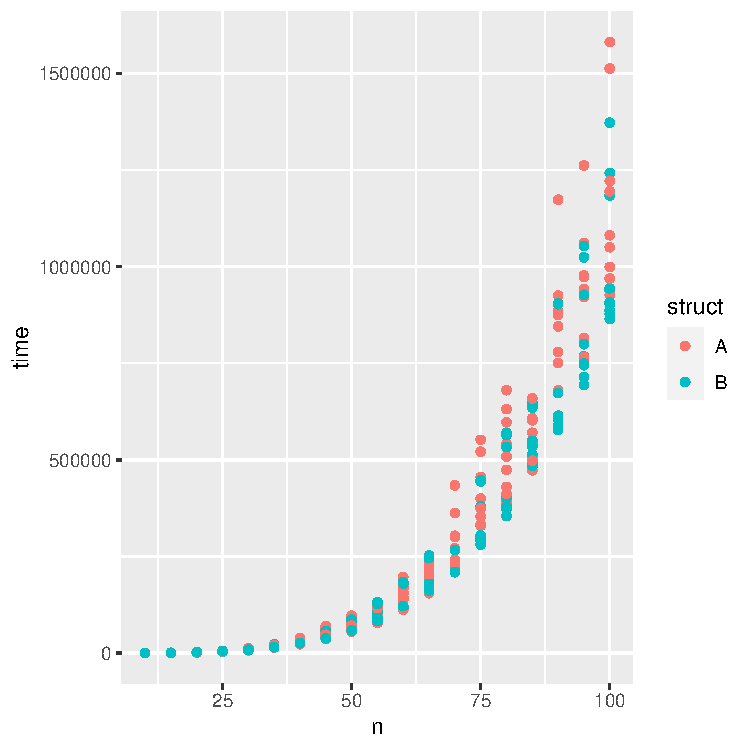
\includegraphics[width=\linewidth]{point.pdf}
            \caption{Все тесты}
        \end{subfigure}%
        \hfill
        \begin{subfigure}[t]{0.475\linewidth}%
            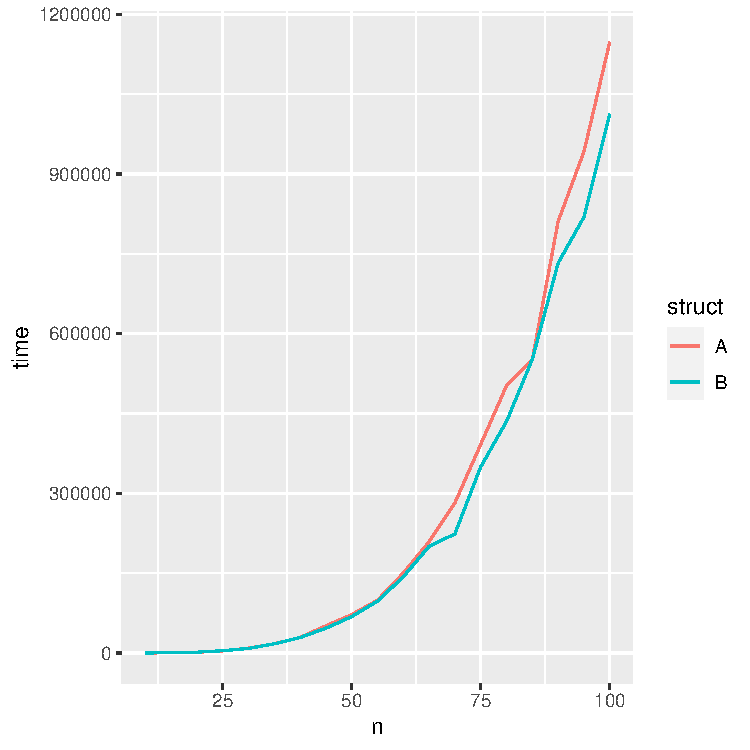
\includegraphics[width=\linewidth]{line.pdf}
            \caption{Среднее тестов}
        \end{subfigure}
        \end{minipage}%
        \hfill
        \begin{minipage}[t]{\columnwidth}% 2nd minipage
        \begin{subfigure}[t]{0.475\linewidth}%
            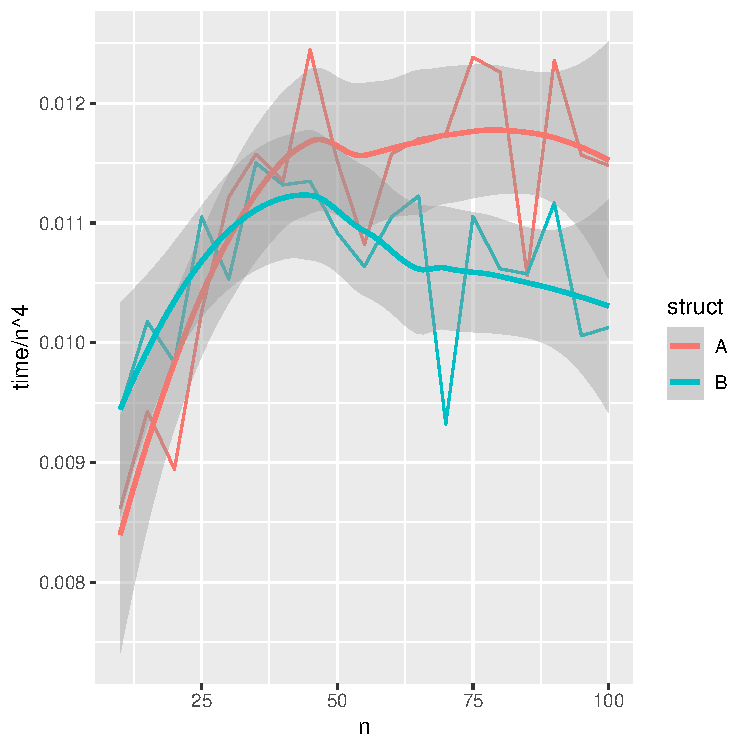
\includegraphics[width=\linewidth]{line_smooth_norm.pdf}
            \caption{Масштабирование по размеру матриц}
        \end{subfigure}%
        \hfill
        \begin{subfigure}[t]{0.475\linewidth}%
            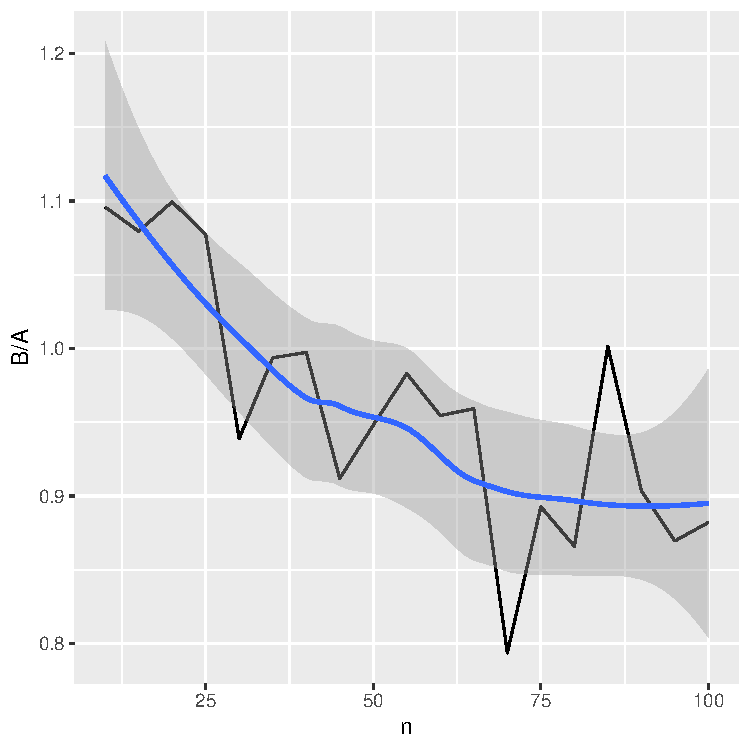
\includegraphics[width=\linewidth]{relation.pdf} 
            \caption{Отношение времени вычисления B и A}
        \end{subfigure}
        \caption{Результаты тестирования.}
        \label{fig:fig1}
        \end{minipage}
    \end{figure*}


    Как видно из графика \ref{fig:fig1}(г), при маленьких размерах матрицы структура A быстрее, а начиная примерно с $n = 30$, структура B становится быстрее. При размерах матрицы $n = 100$ (время вычисления порядка 20 минут) структура B лучше на 10\%.



    % \chapter{Пример решения практической задачи}
        % Задача:
$$C= \begin{pmatrix}
1 & 1/5 & 1/5 & 1 & 1/3\\
5 & 1 & 1/5 & 1/5 & 1\\
5 & 5 & 1 & 1/5 & 1\\
1 & 5 & 5 & 1 & 5\\
3 & 1 & 1 & 1/5 & 1
\end{pmatrix}
$$
$$A_1= \begin{pmatrix}
1 & 3 & 7 & 9\\
1/3 & 1 & 6 & 7\\
1/7 & 1/6 & 1 & 3\\
1/9 & 1/7 & 1/3 & 1
\end{pmatrix}
$$
$$A_2= \begin{pmatrix}
1 & 1/5 & 1/6 & 1/4\\
5 & 1 & 2 & 4\\
6 & 1/2 & 1 & 6\\
4 & 1/4 & 1/6 & 1
\end{pmatrix}
$$
$$A_3= \begin{pmatrix}
1 & 7 & 7 & 1/2\\
1/7 & 1 & 1 & 1/7\\
1/7 & 1 & 1 & 1/7\\
2 & 7 & 7 & 1
\end{pmatrix}
$$
$$A_4= \begin{pmatrix}
1 & 4 & 1/4 & 1/3\\
1/4 & 1 & 1/2 & 3\\
4 & 2 & 1 & 3\\
3 & 1/3 & 1/3 & 1
\end{pmatrix}
$$
$$A_5= \begin{pmatrix}
1 & 1 & 7 & 4\\
1 & 1 & 6 & 3\\
1/7 & 1/6 & 1 & 1/4\\
1/4 & 1/3 & 4 & 1
\end{pmatrix}
$$
Нужные степени матрицы $C$:
$$C^2 = \begin{pmatrix}
1 & 5 & 5 & 1 & 5\\
5 & 1 & 1 & 5 & 5/3\\
25 & 5 & 1 & 5 & 5\\
25 & 25 & 5 & 1 & 5\\
5 & 5 & 1 & 3 & 1
\end{pmatrix}
$$
$$C^3 = \begin{pmatrix}
25 & 25 & 5 & 1 & 5\\
5 & 25 & 25 & 5 & 25\\
25 & 25 & 25 & 25 & 25\\
125 & 25 & 5 & 25 & 25\\
25 & 15 & 15 & 5 & 15
\end{pmatrix}
$$
$$C^4 = \begin{pmatrix}
125 & 25 & 5 & 25 & 25\\
125 & 125 & 25 & 5 & 25\\
125 & 125 & 125 & 25 & 125\\
125 & 125 & 125 & 125 & 125\\
75 & 75 & 25 & 25 & 25
\end{pmatrix}
$$
$$C^5 = \begin{pmatrix}
125 & 125 & 125 & 125 & 125\\
625 & 125 & 25 & 125 & 125\\
625 & 625 & 125 & 125 & 125\\
625 & 625 & 625 & 125 & 625\\
375 & 125 & 125 & 75 & 125
\end{pmatrix}
$$
Спектральный радиус матрицы $C$:
$$\lambda_{C} = \mathrm{tr}C\oplus \dots \oplus \mathrm{tr}^{1/5}(C^{5}) = (125)^{1/4} \approx 3.3437$$
Матрица $\lambda^{-1}C$ и ее степени:
$$(\lambda^{-1}C)^1 = \begin{pmatrix}
(1/125)^{1/4} & (1/78125)^{1/4} & (1/78125)^{1/4} & (1/125)^{1/4} & (1/10125)^{1/4}\\
(5)^{1/4} & (1/125)^{1/4} & (1/78125)^{1/4} & (1/78125)^{1/4} & (1/125)^{1/4}\\
(5)^{1/4} & (5)^{1/4} & (1/125)^{1/4} & (1/78125)^{1/4} & (1/125)^{1/4}\\
(1/125)^{1/4} & (5)^{1/4} & (5)^{1/4} & (1/125)^{1/4} & (5)^{1/4}\\
(81/125)^{1/4} & (1/125)^{1/4} & (1/125)^{1/4} & (1/78125)^{1/4} & (1/125)^{1/4}
\end{pmatrix}
$$
$$(\lambda^{-1}C)^2 = \begin{pmatrix}
(1/15625)^{1/4} & (1/25)^{1/4} & (1/25)^{1/4} & (1/15625)^{1/4} & (1/25)^{1/4}\\
(1/25)^{1/4} & (1/15625)^{1/4} & (1/15625)^{1/4} & (1/25)^{1/4} & (1/2025)^{1/4}\\
(25)^{1/4} & (1/25)^{1/4} & (1/15625)^{1/4} & (1/25)^{1/4} & (1/25)^{1/4}\\
(25)^{1/4} & (25)^{1/4} & (1/25)^{1/4} & (1/15625)^{1/4} & (1/25)^{1/4}\\
(1/25)^{1/4} & (1/25)^{1/4} & (1/15625)^{1/4} & (81/15625)^{1/4} & (1/15625)^{1/4}
\end{pmatrix}
$$
$$(\lambda^{-1}C)^3 = \begin{pmatrix}
(1/5)^{1/4} & (1/5)^{1/4} & (1/3125)^{1/4} & (1/1953125)^{1/4} & (1/3125)^{1/4}\\
(1/3125)^{1/4} & (1/5)^{1/4} & (1/5)^{1/4} & (1/3125)^{1/4} & (1/5)^{1/4}\\
(1/5)^{1/4} & (1/5)^{1/4} & (1/5)^{1/4} & (1/5)^{1/4} & (1/5)^{1/4}\\
(125)^{1/4} & (1/5)^{1/4} & (1/3125)^{1/4} & (1/5)^{1/4} & (1/5)^{1/4}\\
(1/5)^{1/4} & (81/3125)^{1/4} & (81/3125)^{1/4} & (1/3125)^{1/4} & (81/3125)^{1/4}
\end{pmatrix}
$$
$$(\lambda^{-1}C)^4 = \begin{pmatrix}
(1)^{1/4} & (1/625)^{1/4} & (1/390625)^{1/4} & (1/625)^{1/4} & (1/625)^{1/4}\\
(1)^{1/4} & (1)^{1/4} & (1/625)^{1/4} & (1/390625)^{1/4} & (1/625)^{1/4}\\
(1)^{1/4} & (1)^{1/4} & (1)^{1/4} & (1/625)^{1/4} & (1)^{1/4}\\
(1)^{1/4} & (1)^{1/4} & (1)^{1/4} & (1)^{1/4} & (1)^{1/4}\\
(81/625)^{1/4} & (81/625)^{1/4} & (1/625)^{1/4} & (1/625)^{1/4} & (1/625)^{1/4}
\end{pmatrix}
$$
Матрица клини:
$$(\lambda^{-1}C)^* = I \oplus (\lambda^{-1}C)^1 \oplus (\lambda^{-1}C)^2 \oplus (\lambda^{-1}C)^3 \oplus (\lambda^{-1}C)^4 = $$
$$ = \begin{pmatrix}
1 & (1/5)^{1/4} & (1/25)^{1/4} & (1/125)^{1/4} & (1/25)^{1/4}\\
(5)^{1/4} & 1 & (1/5)^{1/4} & (1/25)^{1/4} & (1/5)^{1/4}\\
(25)^{1/4} & (5)^{1/4} & 1 & (1/5)^{1/4} & (1)^{1/4}\\
(125)^{1/4} & (25)^{1/4} & (5)^{1/4} & 1 & (5)^{1/4}\\
(81/125)^{1/4} & (81/625)^{1/4} & (81/3125)^{1/4} & (81/15625)^{1/4} & 1
\end{pmatrix}
$$
Линейно независимые столбцы:
$$P = \begin{pmatrix}
1 & (1/25)^{1/4}\\
(5)^{1/4} & (1/5)^{1/4}\\
(25)^{1/4} & (1)^{1/4}\\
(125)^{1/4} & (5)^{1/4}\\
(81/125)^{1/4} & 1
\end{pmatrix}
$$
$$w_1 = \begin{pmatrix}
(1/125)^{1/4}\\
(1/25)^{1/4}\\
(1/5)^{1/4}\\
(1)^{1/4}\\
(81/15625)^{1/4}
\end{pmatrix}
\qquad w_2 = \begin{pmatrix}
(1/125)^{1/4} & (1/125)^{1/4}\\
(1/25)^{1/4} & (1/25)^{1/4}\\
(1/5)^{1/4} & (1/5)^{1/4}\\
(1)^{1/4} & (1)^{1/4}\\
(1/125)^{1/4} & (1/5)^{1/4}
\end{pmatrix}
$$
$$B = \begin{pmatrix}
(1)^{1/4} & (2401/5)^{1/4} & (2401/5)^{1/4} & (6561/125)^{1/4}\\
(25)^{1/4} & (1)^{1/4} & (1296/125)^{1/4} & (81)^{1/4}\\
(256)^{1/4} & (16)^{1/4} & (1)^{1/4} & (81)^{1/4}\\
(81)^{1/4} & (2401/5)^{1/4} & (2401/5)^{1/4} & (1)^{1/4}
\end{pmatrix}
$$
$$D = \begin{pmatrix}
(1)^{1/4} & (2401/5)^{1/4} & (2401/5)^{1/4} & (6561/125)^{1/4}\\
(25)^{1/4} & (1)^{1/4} & (1296/125)^{1/4} & (81)^{1/4}\\
(256)^{1/4} & (16)^{1/4} & (1)^{1/4} & (81)^{1/4}\\
(81)^{1/4} & (2401/5)^{1/4} & (2401/5)^{1/4} & (1)^{1/4}
\end{pmatrix}
$$
Нужные степени матрицы $B$:
$$B^2 = \begin{pmatrix}
(614656/5)^{1/4} & (15752961/625)^{1/4} & (15752961/625)^{1/4} & (194481/5)^{1/4}\\
(6561)^{1/4} & (194481/5)^{1/4} & (194481/5)^{1/4} & (6561/5)^{1/4}\\
(6561)^{1/4} & (614656/5)^{1/4} & (614656/5)^{1/4} & (1679616/125)^{1/4}\\
(614656/5)^{1/4} & (194481/5)^{1/4} & (194481/5)^{1/4} & (194481/5)^{1/4}
\end{pmatrix}
$$
$$B^3 = \begin{pmatrix}
(4032758016/625)^{1/4} & (1475789056/25)^{1/4} & (1475789056/25)^{1/4} & (4032758016/625)^{1/4}\\
(49787136/5)^{1/4} & (15752961/5)^{1/4} & (15752961/5)^{1/4} & (15752961/5)^{1/4}\\
(157351936/5)^{1/4} & (4032758016/625)^{1/4} & (4032758016/625)^{1/4} & (49787136/5)^{1/4}\\
(49787136/5)^{1/4} & (1475789056/25)^{1/4} & (1475789056/25)^{1/4} & (4032758016/625)^{1/4}
\end{pmatrix}
$$
$$B^4 = \begin{pmatrix}
(377801998336/25)^{1/4} & (9682651996416/3125)^{1/4} & (9682651996416/3125)^{1/4} & (119538913536/25)^{1/4}\\
(4032758016/5)^{1/4} & (119538913536/25)^{1/4} & (119538913536/25)^{1/4} & (326653399296/625)^{1/4}\\
(1032386052096/625)^{1/4} & (377801998336/25)^{1/4} & (377801998336/25)^{1/4} & (1032386052096/625)^{1/4}\\
(377801998336/25)^{1/4} & (119538913536/25)^{1/4} & (119538913536/25)^{1/4} & (119538913536/25)^{1/4}
\end{pmatrix}
$$
Спектральный радиус матрицы $B$:
$$\lambda_{B} = \mathrm{tr}B\oplus \dots \oplus \mathrm{tr}^{1/4}(B^{4}) = (614656/5)^{1/8} \approx 4.32721$$
Матрица $\lambda^{-1}B$ и ее степени:
$$(\lambda^{-1}B)^1 = \begin{pmatrix}
(5/614656)^{1/8} & (2401/1280)^{1/8} & (2401/1280)^{1/8} & (43046721/1920800000)^{1/8}\\
(3125/614656)^{1/8} & (5/614656)^{1/8} & (6561/7503125)^{1/8} & (32805/614656)^{1/8}\\
(1280/2401)^{1/8} & (5/2401)^{1/8} & (5/614656)^{1/8} & (32805/614656)^{1/8}\\
(32805/614656)^{1/8} & (2401/1280)^{1/8} & (2401/1280)^{1/8} & (5/614656)^{1/8}
\end{pmatrix}
$$
$$(\lambda^{-1}B)^2 = \begin{pmatrix}
(1)^{1/8} & (43046721/1024000000)^{1/8} & (43046721/1024000000)^{1/8} & (6561/65536)^{1/8}\\
(1076168025/377801998336)^{1/8} & (6561/65536)^{1/8} & (6561/65536)^{1/8} & (43046721/377801998336)^{1/8}\\
(1076168025/377801998336)^{1/8} & (1)^{1/8} & (1)^{1/8} & (43046721/3603000625)^{1/8}\\
(1)^{1/8} & (6561/65536)^{1/8} & (6561/65536)^{1/8} & (6561/65536)^{1/8}
\end{pmatrix}
$$
$$(\lambda^{-1}B)^3 = \begin{pmatrix}
(43046721/1920800000)^{1/8} & (2401/1280)^{1/8} & (2401/1280)^{1/8} & (43046721/1920800000)^{1/8}\\
(32805/614656)^{1/8} & (215233605/40282095616)^{1/8} & (215233605/40282095616)^{1/8} & (215233605/40282095616)^{1/8}\\
(1280/2401)^{1/8} & (43046721/1920800000)^{1/8} & (43046721/1920800000)^{1/8} & (32805/614656)^{1/8}\\
(32805/614656)^{1/8} & (2401/1280)^{1/8} & (2401/1280)^{1/8} & (43046721/1920800000)^{1/8}
\end{pmatrix}
$$
Матрица клини:
$$(\lambda^{-1}B)^* = I \oplus (\lambda^{-1}B)^1 \oplus (\lambda^{-1}B)^2 \oplus (\lambda^{-1}B)^3 = $$
$$ = \begin{pmatrix}
1 & (2401/1280)^{1/8} & (2401/1280)^{1/8} & (6561/65536)^{1/8}\\
(32805/614656)^{1/8} & 1 & (6561/65536)^{1/8} & (32805/614656)^{1/8}\\
(1280/2401)^{1/8} & (1)^{1/8} & 1 & (32805/614656)^{1/8}\\
(1)^{1/8} & (2401/1280)^{1/8} & (2401/1280)^{1/8} & 1
\end{pmatrix}
$$
Линейно независимые столбцы:
$$P = \begin{pmatrix}
1 & (2401/1280)^{1/8} & (6561/65536)^{1/8}\\
(32805/614656)^{1/8} & 1 & (32805/614656)^{1/8}\\
(1280/2401)^{1/8} & (1)^{1/8} & (32805/614656)^{1/8}\\
(1)^{1/8} & (2401/1280)^{1/8} & 1
\end{pmatrix}
$$
$$w_1 = \begin{pmatrix}
1 & (6561/65536)^{1/8}\\
(32805/614656)^{1/8} & (32805/614656)^{1/8}\\
(1280/2401)^{1/8} & (32805/614656)^{1/8}\\
(1)^{1/8} & (1)^{1/8}
\end{pmatrix}
\qquad w_2 = \begin{pmatrix}
1\\
(1280/2401)^{1/8}\\
(1280/2401)^{1/8}\\
(1)^{1/8}
\end{pmatrix}
$$
Нужные степени матрицы $D$:
$$D^2 = \begin{pmatrix}
(614656/5)^{1/4} & (15752961/625)^{1/4} & (15752961/625)^{1/4} & (194481/5)^{1/4}\\
(6561)^{1/4} & (194481/5)^{1/4} & (194481/5)^{1/4} & (6561/5)^{1/4}\\
(6561)^{1/4} & (614656/5)^{1/4} & (614656/5)^{1/4} & (1679616/125)^{1/4}\\
(614656/5)^{1/4} & (194481/5)^{1/4} & (194481/5)^{1/4} & (194481/5)^{1/4}
\end{pmatrix}
$$
$$D^3 = \begin{pmatrix}
(4032758016/625)^{1/4} & (1475789056/25)^{1/4} & (1475789056/25)^{1/4} & (4032758016/625)^{1/4}\\
(49787136/5)^{1/4} & (15752961/5)^{1/4} & (15752961/5)^{1/4} & (15752961/5)^{1/4}\\
(157351936/5)^{1/4} & (4032758016/625)^{1/4} & (4032758016/625)^{1/4} & (49787136/5)^{1/4}\\
(49787136/5)^{1/4} & (1475789056/25)^{1/4} & (1475789056/25)^{1/4} & (4032758016/625)^{1/4}
\end{pmatrix}
$$
$$D^4 = \begin{pmatrix}
(377801998336/25)^{1/4} & (9682651996416/3125)^{1/4} & (9682651996416/3125)^{1/4} & (119538913536/25)^{1/4}\\
(4032758016/5)^{1/4} & (119538913536/25)^{1/4} & (119538913536/25)^{1/4} & (326653399296/625)^{1/4}\\
(1032386052096/625)^{1/4} & (377801998336/25)^{1/4} & (377801998336/25)^{1/4} & (1032386052096/625)^{1/4}\\
(377801998336/25)^{1/4} & (119538913536/25)^{1/4} & (119538913536/25)^{1/4} & (119538913536/25)^{1/4}
\end{pmatrix}
$$
Спектральный радиус матрицы $D$:
$$\lambda_{D} = \mathrm{tr}D\oplus \dots \oplus \mathrm{tr}^{1/4}(D^{4}) = (614656/5)^{1/8} \approx 4.32721$$
Матрица $\lambda^{-1}D$ и ее степени:
$$(\lambda^{-1}D)^1 = \begin{pmatrix}
(5/614656)^{1/8} & (2401/1280)^{1/8} & (2401/1280)^{1/8} & (43046721/1920800000)^{1/8}\\
(3125/614656)^{1/8} & (5/614656)^{1/8} & (6561/7503125)^{1/8} & (32805/614656)^{1/8}\\
(1280/2401)^{1/8} & (5/2401)^{1/8} & (5/614656)^{1/8} & (32805/614656)^{1/8}\\
(32805/614656)^{1/8} & (2401/1280)^{1/8} & (2401/1280)^{1/8} & (5/614656)^{1/8}
\end{pmatrix}
$$
$$(\lambda^{-1}D)^2 = \begin{pmatrix}
(1)^{1/8} & (43046721/1024000000)^{1/8} & (43046721/1024000000)^{1/8} & (6561/65536)^{1/8}\\
(1076168025/377801998336)^{1/8} & (6561/65536)^{1/8} & (6561/65536)^{1/8} & (43046721/377801998336)^{1/8}\\
(1076168025/377801998336)^{1/8} & (1)^{1/8} & (1)^{1/8} & (43046721/3603000625)^{1/8}\\
(1)^{1/8} & (6561/65536)^{1/8} & (6561/65536)^{1/8} & (6561/65536)^{1/8}
\end{pmatrix}
$$
$$(\lambda^{-1}D)^3 = \begin{pmatrix}
(43046721/1920800000)^{1/8} & (2401/1280)^{1/8} & (2401/1280)^{1/8} & (43046721/1920800000)^{1/8}\\
(32805/614656)^{1/8} & (215233605/40282095616)^{1/8} & (215233605/40282095616)^{1/8} & (215233605/40282095616)^{1/8}\\
(1280/2401)^{1/8} & (43046721/1920800000)^{1/8} & (43046721/1920800000)^{1/8} & (32805/614656)^{1/8}\\
(32805/614656)^{1/8} & (2401/1280)^{1/8} & (2401/1280)^{1/8} & (43046721/1920800000)^{1/8}
\end{pmatrix}
$$
Матрица клини:
$$(\lambda^{-1}D)^* = I \oplus (\lambda^{-1}D)^1 \oplus (\lambda^{-1}D)^2 \oplus (\lambda^{-1}D)^3 = $$
$$ = \begin{pmatrix}
1 & (2401/1280)^{1/8} & (2401/1280)^{1/8} & (6561/65536)^{1/8}\\
(32805/614656)^{1/8} & 1 & (6561/65536)^{1/8} & (32805/614656)^{1/8}\\
(1280/2401)^{1/8} & (1)^{1/8} & 1 & (32805/614656)^{1/8}\\
(1)^{1/8} & (2401/1280)^{1/8} & (2401/1280)^{1/8} & 1
\end{pmatrix}
$$
Линейно независимые столбцы:
$$P = \begin{pmatrix}
1 & (2401/1280)^{1/8} & (6561/65536)^{1/8}\\
(32805/614656)^{1/8} & 1 & (32805/614656)^{1/8}\\
(1280/2401)^{1/8} & (1)^{1/8} & (32805/614656)^{1/8}\\
(1)^{1/8} & (2401/1280)^{1/8} & 1
\end{pmatrix}
$$
$$w_1 = \begin{pmatrix}
1 & (6561/65536)^{1/8}\\
(32805/614656)^{1/8} & (32805/614656)^{1/8}\\
(1280/2401)^{1/8} & (32805/614656)^{1/8}\\
(1)^{1/8} & (1)^{1/8}
\end{pmatrix}
\qquad w_2 = \begin{pmatrix}
1\\
(1280/2401)^{1/8}\\
(1280/2401)^{1/8}\\
(1)^{1/8}
\end{pmatrix}
$$
$$w_{best} = \begin{pmatrix}
1.000000 & 0.750000\\
0.693288 & 0.693288\\
0.924384 & 0.693288\\
1.000000 & 1.000000
\end{pmatrix}
$$
$$w_{worst} = \begin{pmatrix}
1.000000\\
0.924384\\
0.924384\\
1.000000
\end{pmatrix}
$$


    \conclusion

    Для решения многокритериальных задач парных сравнений разработаны модели представления данных, алгоритмы точных вычислений, их программная реализация и проведено сравнение.

    Полученные результаты могут оказаться полезными для решения других задач, где требуется обеспечить точные вычисления, например для задач криптографии.
    
    На языке $\Cpp$ было разработано программное средство \cite{SourceCode}, реализующее описанные выше структуры и аппарат тропической математики.  
    
    \renewcommand{\refname}{}
    \vspace{-25pt}
    \bibliographystyle{ugost2008}
    \bibliography{references}

    % \appendix
    %     \chapter{Исходный код}

    % \renewcommand{\sectionfont}{\normalsize\bfseries}
    % \renewcommand{\theappendixfont}{\normalsize\bfseries}
    % \clearpage
    % \addcontentsline{toc}{chapter}{Приложения}

    % \addcontentsline{toc}{section}{fraction.h}
\begin{lstlisting}[caption=fraction.h\label{listing:fraction}]
#pragma once

#include <string>
#include <assert.h>
#include <iostream>
#include <utility> //pair
#include <numeric> //gcd
#include <cmath>   //pow
#include <cln/integer.h>

class MaxMultiFraction
{
public:
    friend std::string to_string(const MaxMultiFraction &fraction);
    friend std::string to_latex(const MaxMultiFraction &fraction);

    MaxMultiFraction(cln::cl_I numerator, cln::cl_I denominator, uint root = 1)
        : numerator_(numerator),
            denominator_(denominator),
            root_(root)
    {
    }

    MaxMultiFraction(double num = 0)
        : numerator_(1),
            denominator_(1),
            root_(1)
    {
        if (fmod(num, 1) == 0)
        {
            numerator_ = int64_t(num);
        }
        else
        {
            if (fmod(1.0 / num, 1) != 0)
            {
                cout << "fraction constructor error\n"
                        << num << endl;
            }
            assert(fmod(1.0 / num, 1) == 0);
            denominator_ = int64_t(1 / num);
        }
    }

    MaxMultiFraction(string str)
        : numerator_(1),
            denominator_(1),
            root_(1)
    {
        auto pos = str.find("/");
        if (pos == str.npos)
        {
            numerator_ = str.c_str();
        }
        else
        {
            numerator_ = str.substr(0, pos).c_str();
            denominator_ = str.substr(pos + 1).c_str();
        }
    }

    bool operator<(const MaxMultiFraction &other) const
    {
        auto tmp = Transform(*this, other);
        return tmp.first < tmp.second;
    }
    bool operator<=(const MaxMultiFraction &other) const
    {
        auto tmp = Transform(*this, other);
        return tmp.first <= tmp.second;
    }
    bool operator>(const MaxMultiFraction &other) const
    {
        auto tmp = Transform(*this, other);
        return tmp.first > tmp.second;
    }
    bool operator>=(const MaxMultiFraction &other) const
    {
        auto tmp = Transform(*this, other);
        return tmp.first >= tmp.second;
    }
    bool operator==(const MaxMultiFraction &other) const
    {
        auto tmp = Transform(*this, other);
        return tmp.first == tmp.second;
    }
    bool operator!=(const MaxMultiFraction &other) const
    {
        auto tmp = Transform(*this, other);
        return tmp.first != tmp.second;
    }

    MaxMultiFraction operator+=(const MaxMultiFraction &other)
    {
        if (*this < other)
        {
            *this = other;
        }
        return *this;
    }
    MaxMultiFraction operator+(const MaxMultiFraction &other) const
    {
        return MaxMultiFraction(*this) += other;
    }

    MaxMultiFraction operator*=(const MaxMultiFraction &other)
    {
        uint root_gcd = std::gcd(root_, other.root_);
        numerator_ = FastPow(numerator_, other.root_ / root_gcd) *
                        FastPow(other.numerator_, root_ / root_gcd);
        denominator_ = FastPow(denominator_, other.root_ / root_gcd) *
                        FastPow(other.denominator_, root_ / root_gcd);
        root_ *= other.root_ / root_gcd;

        Simplify();

        return *this;
    }
    MaxMultiFraction operator*(const MaxMultiFraction &other) const
    {
        return MaxMultiFraction(*this) *= other;
    }

    MaxMultiFraction operator/=(const MaxMultiFraction &other)
    {
        uint root_gcd = std::gcd(root_, other.root_);
        numerator_ = FastPow(numerator_, other.root_ / root_gcd) *
                        FastPow(other.denominator_, root_ / root_gcd);
        denominator_ = FastPow(denominator_, other.root_ / root_gcd) *
                        FastPow(other.numerator_, root_ / root_gcd);
        root_ *= other.root_ / root_gcd;

        Simplify();

        return *this;
    }
    MaxMultiFraction operator/(const MaxMultiFraction &other) const
    {
        return MaxMultiFraction(*this) /= other;
    }

    MaxMultiFraction Root(uint root) const
    {
        return MaxMultiFraction(numerator_,
                                denominator_,
                                root_ * root)
            .Simplify();
    }
    MaxMultiFraction Pow(uint pow) const
    {
        uint root_pow_gcd = std::gcd(root_, pow);
        pow /= root_pow_gcd;
        return MaxMultiFraction(FastPow(numerator_, pow),
                                FastPow(denominator_, pow),
                                root_ / root_pow_gcd);
    }

    operator double() const
    {
        return std::pow(cln::double_approx(numerator_)
            / cln::double_approx(denominator_), 1.0 / root_);
    }

private:
    cln::cl_I numerator_;
    cln::cl_I denominator_;
    uint root_;

    MaxMultiFraction Simplify()
    {
        cln::cl_I num_den_gcd = cln::gcd(numerator_, denominator_);
        numerator_ = cln::exquo(numerator_, num_den_gcd);
        denominator_ = cln::exquo(denominator_, num_den_gcd);

        return *this;
    }

    cln::cl_I FastPow(cln::cl_I base, cln::cl_I exp) const
    {
        cln::cl_I result = 1;
        while (exp > 0)
        {
            if (cl_I_to_int(exp) & 1)
            {
                result *= base;
            }
            base *= base;
            exp >>= 1;
        }
        return result;
    }

    std::pair<cln::cl_I, cln::cl_I> Transform(const MaxMultiFraction &first, 
                                        const MaxMultiFraction &second) const
    {
        uint gcd_root = std::gcd(first.root_, second.root_);
        return {FastPow(first.numerator_, second.root_ / gcd_root) *
                    FastPow(second.denominator_, first.root_ / gcd_root),
                FastPow(second.numerator_, first.root_ / gcd_root) *
                    FastPow(first.denominator_, second.root_ / gcd_root)};
    }
};

\end{lstlisting}
    % \addcontentsline{toc}{section}{matrix.h}
\begin{lstlisting}[caption=matrix.h\label{listing:matrix}]
#pragma once

#include <vector>
#include <assert.h>
#include <iostream>
#include <string>

using namespace std;

template <typename T>
class Matrix;
template <typename T>
Matrix<T> Identity(uint size);
template <typename T>
Matrix<T> Ones(uint rows, uint cols);

template <typename T>
class Matrix
{
public:
    Matrix(uint rows, uint cols, T value = 0)
        : matrix_(rows, std::vector<T>(cols, value)) {}
    Matrix(const std::vector<std::vector<T>> &matrix)
        : matrix_(matrix) {}
    Matrix(std::initializer_list<std::vector<T>> matrix)
        : matrix_(matrix)
    {
        // std::cout << "initializer_list T" << std::endl;

        for (uint i = 0; i < rows(); i++)
        {
            assert(cols() == matrix_[i].size());
        }
    }
    template <typename U>
    Matrix(const Matrix<U> &other) : Matrix(other.rows(), other.cols())
    {
        // std::cout << "Matrix U" << std::endl;

        for (uint i = 0; i < rows(); i++)
        {
            for (uint j = 0; j < cols(); j++)
            {
                matrix_[i][j] = other[i][j];
            }
        }
    }

    std::vector<T> &operator[](uint i)
    {
        return matrix_[i];
    }
    const std::vector<T> &operator[](uint i) const
    {
        return matrix_[i];
    }

    Matrix operator+=(const Matrix &other)
    {
        assert(rows() == other.rows());
        assert(cols() == other.cols());
        for (uint i = 0; i < rows(); i++)
        {
            for (uint j = 0; j < cols(); j++)
            {
                matrix_[i][j] += other[i][j];
            }
        }
        return *this;
    }
    Matrix operator+(const Matrix &other) const
    {
        return Matrix(*this) += other;
    }

    Matrix operator-() const
    {
        Matrix result(rows(), cols());
        for (uint i = 0; i < rows(); i++)
        {
            for (uint j = 0; j < cols(); j++)
            {
                result[i][j] = -matrix_[i][j];
            }
        }
        return result;
    }
    Matrix operator-=(const Matrix &other)
    {
        assert(rows() == other.rows());
        assert(cols() == other.cols());
        for (uint i = 0; i < rows(); i++)
        {
            for (uint j = 0; j < cols(); j++)
            {
                matrix_[i][j] -= other[i][j];
            }
        }
        return *this;
    }
    Matrix operator-(const Matrix &other) const
    {
        return Matrix(*this) -= other;
    }

    Matrix operator*=(const Matrix &other)
    {
        assert(cols() == other.rows());
        Matrix result(rows(), other.cols());
        for (uint i = 0; i < result.rows(); i++)
        {
            for (uint j = 0; j < result.cols(); j++)
            {
                for (uint k = 0; k < cols(); k++)
                {
                    result[i][j] += matrix_[i][k] * other[k][j];
                }
            }
        }
        matrix_ = std::move(result.matrix_);
        return *this;
    }
    Matrix operator*(const Matrix &other) const
    {
        return Matrix(*this) *= other;
    }

    Matrix operator*=(const T &scalar)
    {
        for (uint i = 0; i < rows(); i++)
        {
            for (uint j = 0; j < cols(); j++)
            {
                matrix_[i][j] *= scalar;
            }
        }
        return *this;
    }
    Matrix operator*(const T &scalar) const
    {
        return Matrix(*this) *= scalar;
    }

    Matrix operator/=(const T &scalar)
    {
        for (uint i = 0; i < rows(); i++)
        {
            for (uint j = 0; j < cols(); j++)
            {
                matrix_[i][j] /= scalar;
            }
        }
        return *this;
    }
    Matrix operator/(const T &scalar) const
    {
        return Matrix(*this) /= scalar;
    }

    Matrix Transpose() const
    {
        Matrix result(cols(), rows());
        for (uint i = 0; i < rows(); i++)
        {
            for (uint j = 0; j < cols(); j++)
            {
                result[j][i] = (matrix_[i][j] == T{0} ? T{0}
                                                      : T{1} / matrix_[i][j]);
            }
        }
        return result;
    }

    T Trace() const
    {
        assert(rows() == cols());
        T result;
        for (uint i = 0; i < cols(); i++)
        {
            result += matrix_[i][i];
        }
        return result;
    }

    T Determinant() const
    {
        T result{Trace()};
        Matrix tmp(*this);
        for (uint i = 1; i < cols(); i++)
        {
            tmp *= *this;
            result += tmp.Trace();
        }
        return result;
    }

    T SpectralRadius() const
    {
        T result{Trace()};
        Matrix tmp(*this);
        for (uint i = 2; i <= cols(); i++)
        {
            tmp *= *this;
            result += tmp.Trace().Root(i);
        }
        return result;
    }

    Matrix Kleene() const
    {
        Matrix tmp{*this};
        Matrix result{Identity<T>(cols())};
        for (uint i = 1; i < cols(); i++)
        {
            result += tmp;
            tmp *= *this;
        }
        return result;
    }

    bool isLinearlyDependent(const Matrix &b)
    {
        assert(b.cols() == 1);
        Matrix &A = *this;
        Matrix result((A * (b.Transpose() * A).Transpose()).Transpose() * b);

        return result[0][0] == T{1};
    }

    Matrix Span()
    {
        Matrix result(getCol(0));
        for (uint j = 1; j < cols(); j++)
        {
            auto tmp = getCol(j);
            if (!result.isLinearlyDependent(tmp))
            {
                result.cbind(tmp);
            }
        }
        return result;
    }

    Matrix BestVector()
    {
        T lambda = SpectralRadius();
        Matrix P((*this / lambda).Kleene().Span());

        // uint k = 0;
        vector<uint> k;
        T max_value = -1;
        for (uint j = 0; j < P.cols(); j++)
        {
            Matrix col_j(P.getCol(j));
            T tmp = (col_j * col_j.Transpose()).sum();
            if (tmp > max_value)
            {
                // k = j;
                k.clear();
                max_value = tmp;
            }
            if (tmp == max_value)
            {
                k.push_back(j);
            }
        }
        vector<uint> l(k.size(), 0);
        for (uint it = 0; it < k.size(); it++)
        {
            for (uint i = 0; i < P.rows(); i++)
            {
                if (P[i][k[it]] < P[l[it]][k[it]])
                {
                    l[it] = i;
                }
            }
        }

        Matrix result(P * (Identity<T>(P.cols()) +
                            P.filter(l[0], k[0]).Transpose() * P));
        for (uint i = 1; i < k.size(); i++)
        {
            result.cbind(P * (Identity<T>(P.cols()) +
                                P.filter(l[1], k[1]).Transpose() * P));
        }

        return result.Span().normCol();
    }

    Matrix WorstVector()
    {
        T lambda(SpectralRadius());
        Matrix kleene((*this / lambda).Kleene());
        T Delta = kleene.sum();
    
        return (Matrix(rows(), cols(), T{1} / Delta)
                + *this / lambda).Kleene().Span().normCol();
    }

    Matrix cbind(const Matrix &other)
    {
        assert(rows() == other.rows());
        for (uint i = 0; i < rows(); i++)
        {
            matrix_[i].insert(matrix_[i].end(), other[i].begin(),
                                                other[i].end());
        }
        return *this;
    }

    Matrix rbind(const Matrix &other)
    {
        assert(cols() == other.cols());
        matrix_.insert(matrix_.end(), other.matrix_.begin(),
                                      other.matrix_.end());
        return *this;
    }

    Matrix getCol(uint j)
    {
        assert(j < cols());
        Matrix result(rows(), 1);
        for (uint i = 0; i < rows(); i++)
        {
            result[i][0] = matrix_[i][j];
        }
        return result;
    }

    Matrix filter(uint i, uint j) const
    {
        assert(i < rows());
        assert(j < cols());
        Matrix result(rows(), cols());
        result[i][j] = (*this)[i][j];
        return result;
    }

    Matrix norm()
    {
        return *this / sum();
    }

    Matrix normCol()
    {
        Matrix result(*this);
        for (uint col = 0; col < result.cols(); col++)
        {
            T max_in_col;
            for (uint row = 0; row < result.rows(); row++)
            {
                max_in_col += result[row][col];
            }
            for (uint row = 0; row < result.rows(); row++)
            {
                result[row][col] /= max_in_col;
            }
        }
        return result;
    }

    T sum()
    {
        return (Ones<T>(1, rows()) * (*this) * Ones<T>(cols(), 1))[0][0];
    }

    uint rows() const
    {
        return matrix_.size();
    }
    uint cols() const
    {
        return matrix_.front().size();
    }

private:
    std::vector<std::vector<T>> matrix_;
};

template <typename T>
Matrix<T> operator*(const T &scalar, const Matrix<T> &matrix)
{
    return Matrix(matrix) *= scalar;
}

template <typename T>
Matrix<T> Identity(uint size)
{
    Matrix<T> result(size, size, T{0});
    for (uint i = 0; i < size; i++)
    {
        result[i][i] = T{1};
    }
    return result;
}

template <typename T>
Matrix<T> Ones(uint rows, uint cols)
{
    Matrix<T> result(rows, cols, T{1});
    return result;
}
    
\end{lstlisting}
    % \addcontentsline{toc}{section}{to\_latex.h}
\begin{lstlisting}[caption=to\_latex.h\label{listing:to_latex}]
#pragma once

#include <iostream>
#include <string>
#include <sstream>
#include "matrix.h"
#include "fraction.h"
#include <cln/integer_io.h>
#include <eigen3/Eigen/Dense>

using std::to_string;

std::string equation(std::string str)
{
    // return "\\begin{equation*}\n" +
    //        str +
    //        "\\end{equation*}";

    return "$$" + str + "$$";
}

template <typename T>
std::ostream &operator<<(std::ostream &out, const Matrix<T> &matrix)
{
    std::cout << to_string(matrix) << std::endl;
    return out;
}

std::ostream &operator<<(std::ostream &out, const MaxMultiFraction &fraction)
{
    std::cout << to_string(fraction);
    return out;
}

template <typename T>
std::string to_string(const Matrix<T> &matrix)
{
    std::string result;
    for (uint i = 0; i < matrix.rows(); i++)
    {
        if (i != 0)
        {
            result += "\n";
        }
        for (uint j = 0; j < matrix.cols(); j++)
        {
            if (j != 0)
            {
                result += " ";
            }
            result += to_string(matrix[i][j]);
        }
    }
    return result;
}

std::string to_string(const cln::cl_I &integer)
{
    std::stringstream ss;
    cln::print_integer(ss, 10, integer);

    return ss.str();
}

std::string to_string(const MaxMultiFraction &fraction)
{
    std::string result = to_string(fraction.numerator_);
    if (fraction.denominator_ != 1)
    {
        result += "/";
        result += to_string(fraction.denominator_);
    }

    if (fraction.root_ != 1)
    {
        result = "(" + result + ")^(1/" + to_string(fraction.root_) + ")";
    }
    return result;
}

template <typename T>
std::string to_latex(const T &obj, std::string name = "")
{
    return name + (name != "" ? " = " : "") + to_string(obj);
}

template <typename T>
std::string to_latex(const Matrix<T> &matrix)
{
    std::string result;
    result += "\\begin{pmatrix}\n";
    for (uint i = 0; i < matrix.rows(); i++)
    {
        if (i != 0)
        {
            result += "\\\\\n";
        }
        for (uint j = 0; j < matrix.cols(); j++)
        {
            if (j != 0)
            {
                result += " & ";
            }
            result += to_latex(matrix[i][j]);
        }
    }
    result += "\n\\end{pmatrix}\n";

    return result;
}

// template <>
std::string to_latex(const MaxMultiFraction &fraction)
{
    std::string result = to_string(fraction.numerator_);
    if (fraction.denominator_ != 1)
    {
        result = result + "/" + to_string(fraction.denominator_);
    }

    if (fraction.root_ != 1)
    {
        result = "(" + result + ")^{1/" + to_string(fraction.root_) + "}";
    }
    return result;
}

// template <typename T>
// template <>
std::string to_latex(const Eigen::MatrixXd &matrix)
{
    std::string result;
    result += "\\begin{pmatrix}\n";
    for (uint i = 0; i < matrix.rows(); i++)
    {
        if (i != 0)
        {
            result += "\\\\\n";
        }
        for (uint j = 0; j < matrix.cols(); j++)
        {
            if (j != 0)
            {
                result += " & ";
            }
            result += to_latex(matrix(i, j));
        }
    }
    result += "\n\\end{pmatrix}\n";

    return result;
}

// template <typename scalar>
std::string to_latex(const Eigen::VectorXd &vector)
{
    std::string result;
    result += "\\begin{pmatrix}\n";
    for (uint i = 0; i < vector.rows(); i++)
    {
        if (i != 0)
        {
            result += "\\\\\n";
        }
        result += to_latex(vector(i));
    }
    result += "\n\\end{pmatrix}\n";

    return result;
}
\end{lstlisting}

    % \begin{lstlisting}
% \begin{lstlisting}[style={CppCodeStyle}]
#include <iostream>
#include "matrix.h"
#include "fraction.h"
#include "to_latex.h"
#include "string"
#include "fstream"
#include <math.h>

#include <eigen3/Eigen/Dense>

typedef MaxMultiFraction Fraction;

ifstream input;
ofstream output;

using namespace std;

Eigen::VectorXd MainVector(Eigen::MatrixXd &matrix)
{
    Eigen::EigenSolver<Eigen::MatrixXd> es(matrix);

    Eigen::VectorXd eigen_values = es.eigenvalues().real();

    uint max_id = 0;
    for (uint i = 1; i < eigen_values.size(); i++)
    {
        max_id = eigen_values[i] > eigen_values[max_id] ? i : max_id;
    }

    // output << "The main eigenvector of the matrix is:\n"
    //      << es.eigenvectors().col(max_id).real() << endl;
    Eigen::VectorXd result = es.eigenvectors().col(max_id).real();
    result /= result.sum();
    return result;
}

void HierarchyAnalysisMethod(Eigen::MatrixXd &C, vector<Eigen::MatrixXd> &A)
{
    Eigen::VectorXd main_vector_C = MainVector(C);

    Eigen::MatrixXd main_vectors_A(A[0].rows(), C.cols());

    for (uint i = 0; i < A.size(); i++)
    {
        main_vectors_A.col(i) = MainVector(A[i]);
    }

    Eigen::VectorXd result = main_vectors_A * main_vector_C;
    result /= result.maxCoeff();
    Eigen::VectorXd result_sum = result / result.sum();

    output << "Главный собственный вектор матрицы $C$\n"
           << equation(to_latex(main_vector_C)) << endl
           << "Главные собственные вектора матриц $A_i$\n"
           << equation(to_latex(main_vectors_A)) << endl
           << "Нормированный по сумме вектор приоритетов\n"
           << equation(to_latex(result_sum)) << endl
           << "Нормированный по максимуму вектор приоритетов\n"
           << equation(to_latex(result)) << endl;
}

Eigen::VectorXd WeightedGeometricMean(Eigen::MatrixXd &matrix)
{
    Eigen::VectorXd result(matrix.rows());
    for (uint i = 0; i < matrix.rows(); i++)
    {
        result(i) = 1;
        for (uint j = 0; j < matrix.cols(); j++)
        {
            result(i) *= matrix(i, j);
        }
        result(i) = pow(result(i), 1.0 / matrix.cols());
    }
    return result;
}

void WeightedGeometricMeanMethod(Eigen::MatrixXd &C, vector<Eigen::MatrixXd> &A)
{
    Eigen::VectorXd weighted_geometric_mean_C = WeightedGeometricMean(C);
    weighted_geometric_mean_C /= weighted_geometric_mean_C.sum();

    Eigen::MatrixXd weighted_geometric_means_A(A[0].rows(), C.cols());

    for (uint i = 0; i < A.size(); i++)
    {
        weighted_geometric_means_A.col(i) = WeightedGeometricMean(A[i]);
    }

    // m.array().log()).matrix();

    Eigen::VectorXd result = (weighted_geometric_means_A.array().log().matrix() * weighted_geometric_mean_C).array().exp().matrix();
    result /= result.maxCoeff();

    output << "Взвешенный по сумме геометрический средний вектор матрицы $C$\n"
           << weighted_geometric_mean_C << endl
           << "Геометрические средние вектора матриц $A_i$\n"
           << weighted_geometric_means_A << endl
           << "Нормированный по сумме вектор приоритетов\n"
           << result / result.sum() << endl
           << "Нормированный по максимуму вектор приоритетов\n"
           << result << endl;
}

void CommonPart(Matrix<Fraction> &C, string matrix_name)
{
    output << "Нужные степени матрицы $" + matrix_name + "$:\n";
    auto tmp(C);
    uint n = C.cols();
    for (uint i = 2; i <= n; i++)
    {
        tmp = tmp * C;
        output << "$$" + matrix_name + "^" << i << " = "
               << to_latex(tmp) << "$$\n";
    }

    output << "Спектральный радиус матрицы $" + matrix_name + "$:\n";
    output << "$$\\lambda_{" + matrix_name + "} = \\mathrm{tr}" + matrix_name + "\\oplus \\dots \\oplus \\mathrm{tr}^{1/" << n << "}(" + matrix_name + "^{" << n << "}) = " + to_latex(C.SpectralRadius()) + " \\approx " << double(C.SpectralRadius()) << "$$\n";

    output << "Матрица $\\lambda^{-1}" + matrix_name + "$ и ее степени:\n";
    tmp = C / C.SpectralRadius();
    auto tmp2(tmp);
    for (uint i = 1; i < n; i++)
    {
        output << "$$(\\lambda^{-1}" + matrix_name + ")^" << i << " = "
               << to_latex(tmp2) << "$$\n";
        tmp2 = tmp2 * tmp;
    }

    output << "Матрица клини:\n";
    output << "$$(\\lambda^{-1}" + matrix_name + ")^* = I";
    for (uint i = 1; i < n; i++)
    {
        output << " \\oplus (\\lambda^{-1}" + matrix_name + ")^" << i;
    }
    output << " = $$\n$$ = " << to_latex((C / C.SpectralRadius()).Kleene()) << "$$\n";

    output << "Линейно независимые столбцы:\n";
    output << "$$P = " << to_latex((C / C.SpectralRadius()).Kleene().Span()) << "$$\n";

    output << "$$w_1 = "
           << to_latex(C.BestVector())
           << "\\qquad w_2 = "
           << to_latex(C.WorstVector()) << "$$\n";
}

void MinMaxLogChebyshevApproximationMethod(Matrix<Fraction> &C, vector<Matrix<Fraction>> &A)
{
    CommonPart(C, "C");

    auto best_vector_combination(C.BestVector());

    Matrix<Fraction> best_combination(A[0].rows(), A[0].cols(), 0);

    for (uint i = 0; i < A.size(); i++)
    {
        best_combination = best_combination + A[i] * best_vector_combination[i][0];
    }

    auto worst_vector_combination(C.WorstVector());

    Matrix<Fraction> worst_combination(A[0].rows(), A[0].cols(), 0);

    for (uint i = 0; i < A.size(); i++)
    {
        worst_combination = worst_combination + A[i] * worst_vector_combination[i][0];
    }

    output << "$$B = " << to_latex(best_combination) << "$$\n";
    output << "$$D = " << to_latex(worst_combination) << "$$\n";

    CommonPart(best_combination, "B");

    CommonPart(worst_combination, "D");

    output << "$$w_{best} = " << to_latex(Matrix<double>(best_combination.BestVector())) << "$$\n";
    output << "$$w_{worst} = " << to_latex(Matrix<double>(worst_combination.WorstVector())) << "$$\n";

    // auto best_vector(C.BestVector());
    // auto worst_vector(C.WorstVector());
    // output << best_vector << worst_vector << endl;
}

Matrix<Fraction> InputMatrix(uint size)
{
    Matrix<Fraction> result(size, size);
    for (uint i = 0; i < size; i++)
    {
        for (uint j = 0; j < size; j++)
        {
            string tmp;
            input >> tmp;
            if (tmp == "")
            {
                input >> tmp;
            }
            result[i][j] = tmp;
        }
    }
    return result;
}

Eigen::MatrixXd CopyMatrix(Matrix<Fraction> &matrix)
{
    Eigen::MatrixXd result(matrix.cols(), matrix.rows());
    for (uint i = 0; i < matrix.cols(); i++)
    {
        for (uint j = 0; j < matrix.rows(); j++)
        {
            result(i, j) = matrix[i][j];
        }
    }
    return result;
}

int main(int argc, char *argv[])
{
    string input_file = "text.txt";
    if (argc >= 2)
    {
        input_file = argv[1];
    }

    input.open(input_file);

    int criteria_num;
    int alternatives_num;

    input >> criteria_num >> alternatives_num;

    Matrix<Fraction> C = InputMatrix(criteria_num);
    Eigen::MatrixXd C_ = CopyMatrix(C);
    vector<Matrix<Fraction>> A;
    vector<Eigen::MatrixXd> A_;

    for (int i = 0; i < criteria_num; i++)
    {
        A.push_back(InputMatrix(alternatives_num));
        A_.push_back(CopyMatrix(A[i]));
    }

    input.close();

    string output_file = "result_" + input_file;
    if (argc >= 3)
    {
        output_file = argv[2];
    }
    output.open(output_file);

    output << "Задача:\n";

    output << "$$C= " << to_latex(C) << "$$\n";
    for (uint i = 0; i < A.size(); i++)
    {
        output << "$$A_" << i + 1 << "= " << to_latex(A[i]) << "$$\n";
    }

    // HierarchyAnalysisMethod(C_, A_);
    // WeightedGeometricMeanMethod(C_, A_);
    MinMaxLogChebyshevApproximationMethod(C, A);

    output.close();

    return 0;
}
\end{lstlisting}


\end{document}